\documentclass[11pt]{paper}
\usepackage{fullpage}
\usepackage{graphicx}
\usepackage{palatino}
\usepackage{fancyhdr}
\usepackage{draftwatermark}
\usepackage{enumitem}
\setlist{nolistsep}

\renewcommand{\headheight}{0.4in}
\setlength{\headsep}{0.1in}

\setlength{\headwidth}{\textwidth}
\fancyhead[R]{\footnotesize m-labs.hk}
\fancyhead[L]{
   
\includegraphics[height=0.17in]{m_labs_logo.pdf}
}
\chead{}
\rfoot{}
\cfoot{\thepage}
\lfoot{}\pagestyle{fancy}

\begin{document}

\title{ARTIQ hardware proposal}
\author{S\'ebastien Bourdeauducq, Robert J\"ordens (M-Labs)}

\maketitle

\section{Background and objectives}
Control electronics used in many trapped-ion and other quantum physics experiments suffers from a number of problems. In general, an ad-hoc solution is hastily put together in-house without enough consideration about good design, reproducibility, testing and documentation. This makes those systems unreliable, fragile, and difficult to use and maintain. It also duplicates work in different laboratories. In addition, the performance and features of the existing systems (e.g.\ regarding pulse shaping abilities) is becoming insufficient for some experiments.

To alleviate those problems, M-Labs wish to propose high-quality and turnkey control hardware, which should be in particular:
\begin{itemize}
\item reproducible and open
\item flexible and modular
\item well tested
\item well supported by the ARTIQ control software
\end{itemize}

This document describes the desired components and features of this system.

We thank Joe Britton (ARL), Grzegorz Kasprowicz (Creotech/Warsaw University of Technology), David Leibrandt (NIST), and Daniel Slichter (NIST) for their valuable input.

\section{System overview}

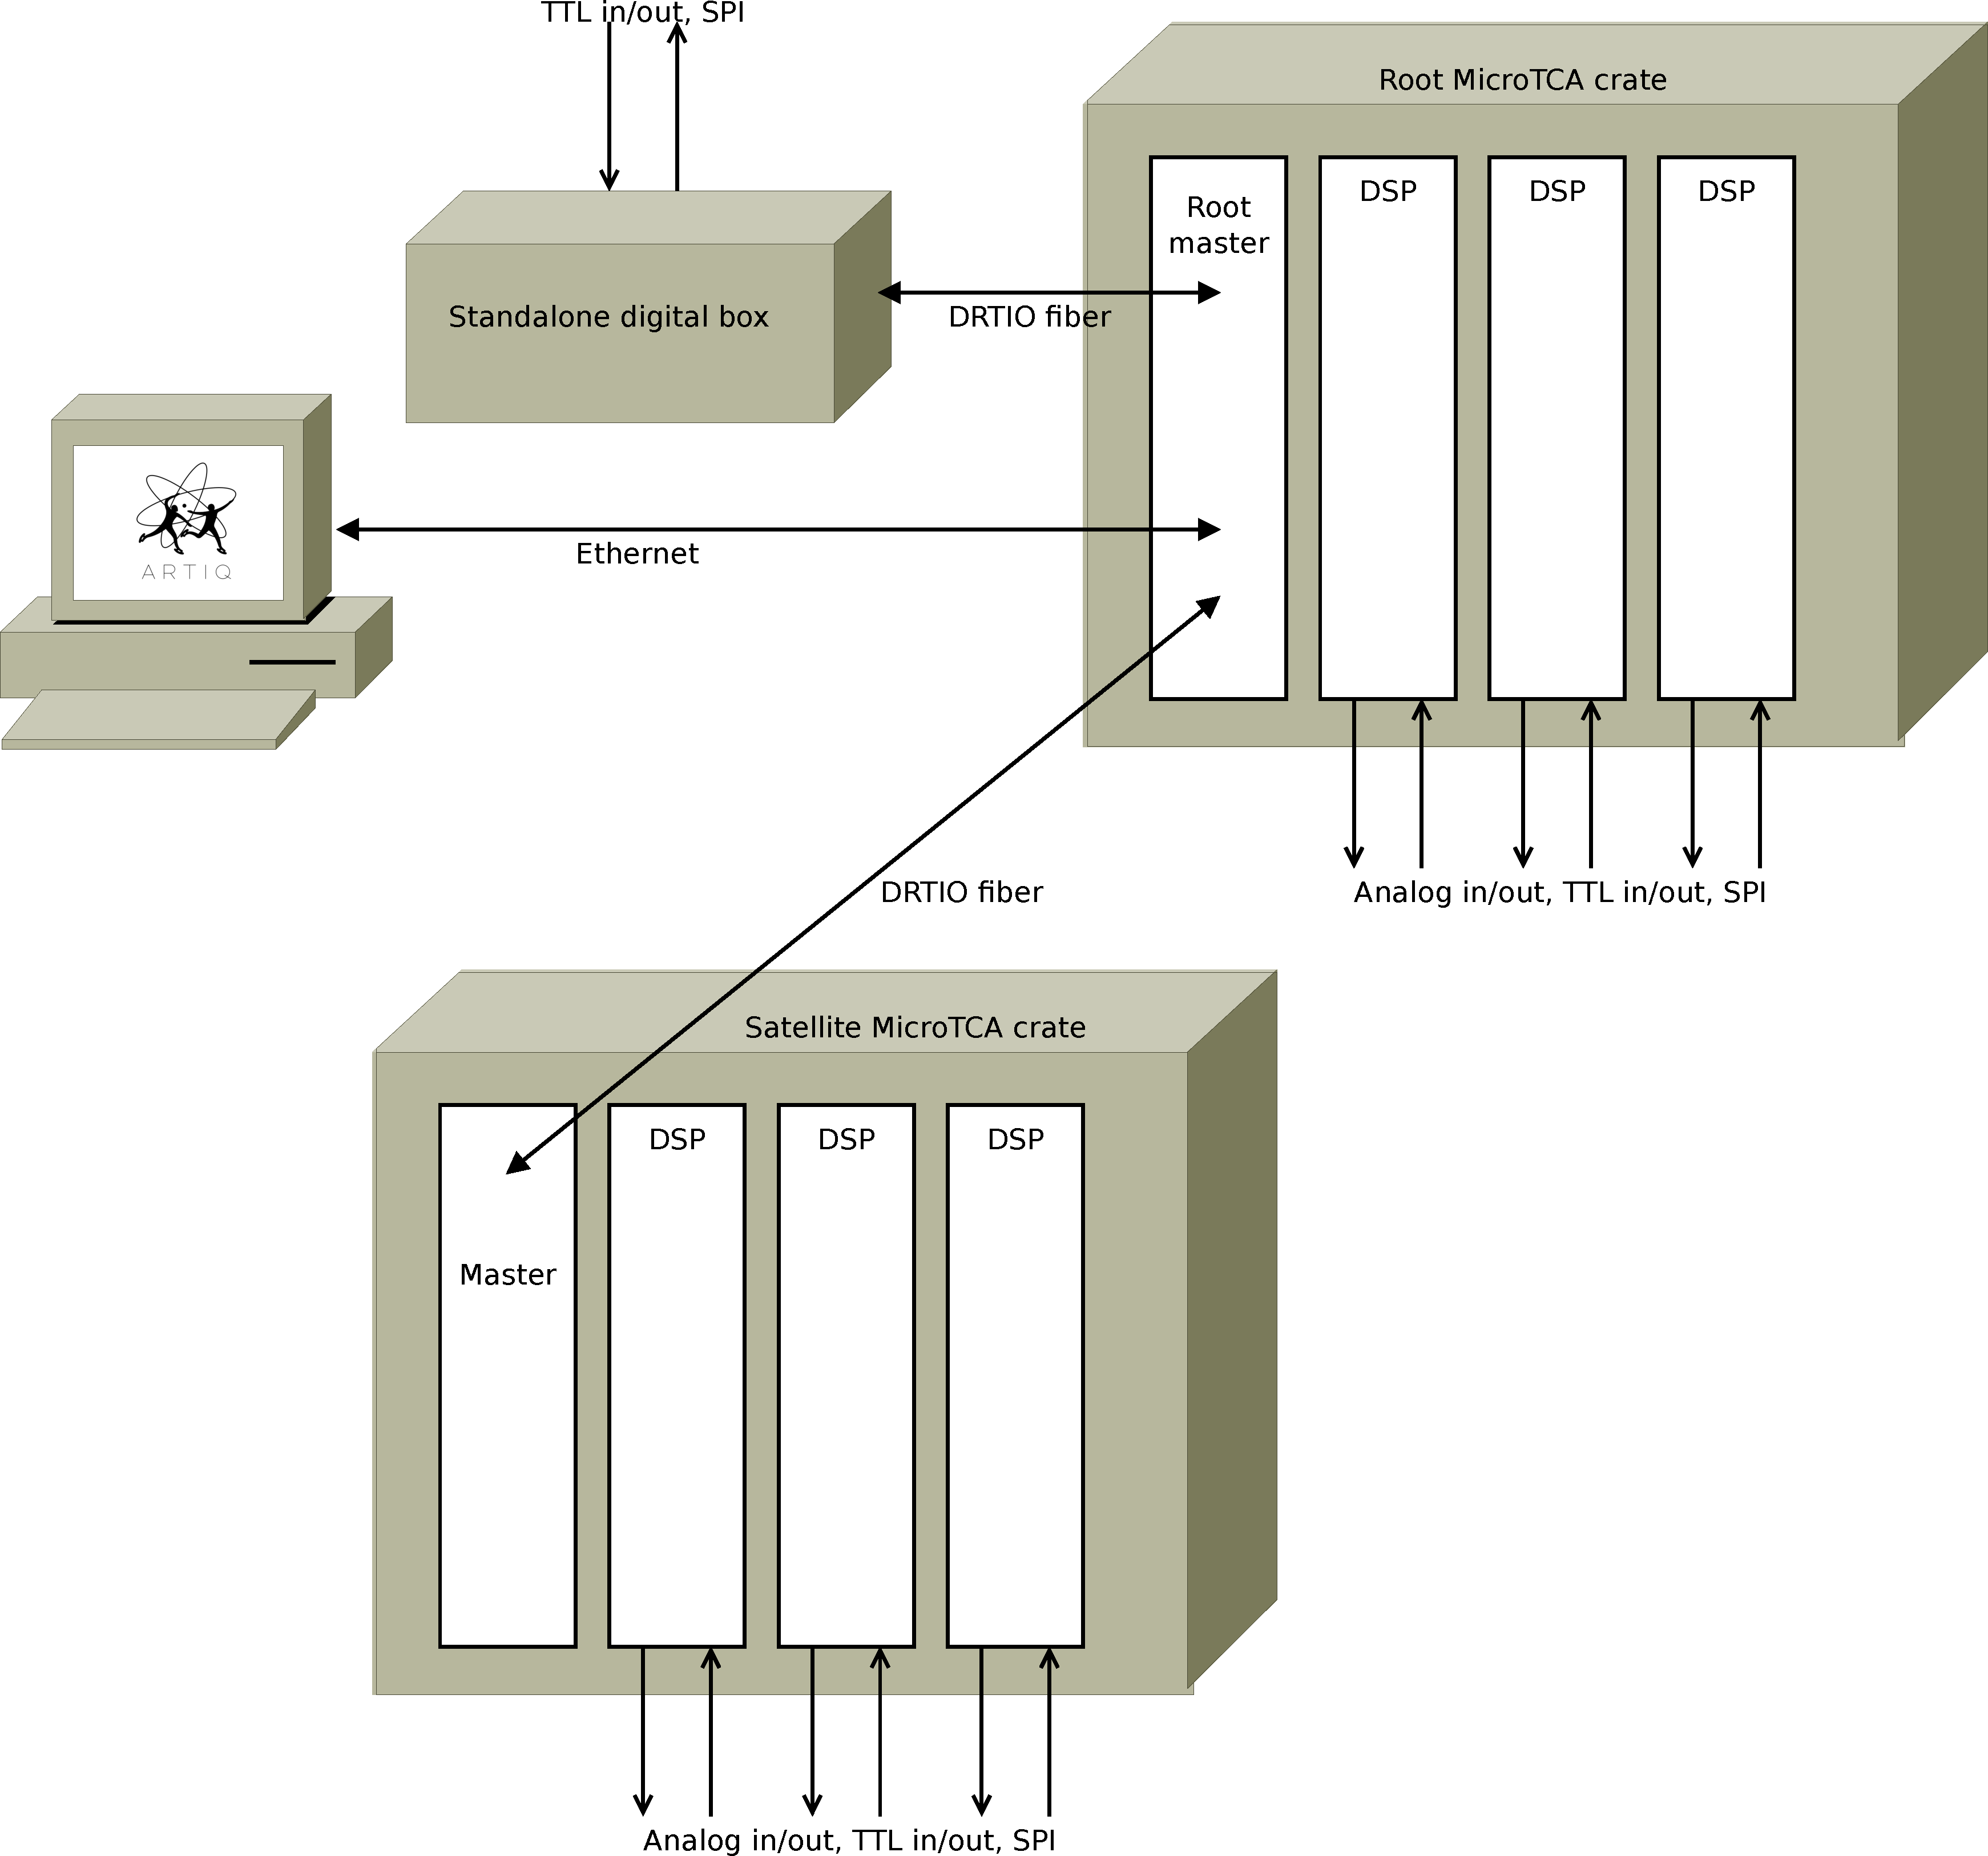
\includegraphics[width=\textwidth]{overview.pdf}

\section{Crates}
The crates are compatible with the MicroTCA standard, and contain a power supply, cooling fans, a backplane (star topology), and AMCs. In order to save space, and to keep all connectors on the same side, RTMs (MicroTCA.4) are not used and the crate should be chosen accordingly.

MicroTCA specifies a complicated ``IPMI'' management system. For compatibility reasons with other MicroTCA systems, the necessary hardware (a microcontroller circuit) should be present on the AMCs, but IPMI should otherwise be ignored as much as possible e.g.\ by keeping the power supplies on at all times.

The gateware/runtime upgrade mechanisms for the hardware components are TBD. A possibility is to send firmware binaries over the fiber or Ethernet for the FPGAs to write into their flash and reboot themselves, which is relatively simple and does not require additional hardware. Another possibility is to have a ``bootloader'' bitstream in flash that downloads the final bitstream ultimately from the control PC through the fiber/Ethernet network. But depending on the FPGA used, this solution may require an additional CPLD/small FPGA and SDRAM/PSRAM to buffer the final bitstream.

\section{Master boards}
A master board is a MicroTCA Carrier Hub (MCH) that:
\begin{itemize}
\item distributes DRTIO commands to the other cards in the crate over the MicroTCA backplane (star topology)
\item distributes DRTIO commands to other crates
\item receives commands from another master board or the control PC
\end{itemize}

It has TBD SFPs on its front panel that are used for connecting to other devices (another master board, TTL box, ...) over raw fiber optics, or to the control PC over Ethernet. The same fiber optic links may also be used for time transfer.

A special master board is the root master, which has the same role as the current core device in ARTIQ. It uses the same hardware as other master boards, but one of its SFPs is populated with a Ethernet PHY that is used to communicate with the control PC.

A master board includes clock recovery and cleanup circuitry, and can be used to clock the other boards in the crate. A master board also includes a SMA clock input connector on its front panel, in case the clock recovered from SFP is not of sufficient quality for the application, and for clocking the root master.

The FPGA used in master boards is TBD.

\section{DSP boards}
The DSP boards are AMC cards that contain a FPGA, fast SDRAM (e.g.\ DDR3 or DDR4), two synchronized JESD204 multi-channel high-speed DACs (AD9154, 8 channels in total) and two synchronized JESD204 ADCs (AD9656, 8 channels in total).

In case of difficulties with board layout, the number of ADC channels may be reduced.

The DAC and ADC channels are sent to a FMC connector that can receive analog cards that contain devices such as RF mixers, and have their own front panel connectors. The purpose of using FMC here is to take advantage of the mechanical work that has already been done to support traditional digital FMC cards.

The FMC also has digital pins that can be used to control the analog cards. To improve signal quality, pins near analog signals should be grounded.

DSP boards can be clocked from the backplane, or from a dedicated SMA connector on their front panel. High-quality clock distribution systems using semi-rigid coaxial cables can be used for particularly sensitive applications.

Remaining space on the front panel of the AMC is used for TTL signals over TBD connectors.

DSP boards receive high level DRTIO commands from the backplane, and synthesize, buffer or process waveforms using their FPGA and SDRAM.

The FPGA used in DSP boards is TBD.

\section{Analog FMC cards}
\subsection{Breakout card}
The breakout card gives direct access to the DAC and ADC signals using SMA connectors on its front panel.

\subsection{Others}
TBD

\section{Standalone digital boxes}
The standalone digital boxes receive DRTIO commands (and possibly time) over a SFP and fiber connected to a master card, and generate and receive TTL pulses and digitally control devices such as SPI integrated circuits. They have TBD SMA connectors and TBD RJ45 connectors that can be connected to e.g.\ SPI devices. They contain their own power supply.

The digital boxes also have a dedicated clock input SMA connector, that can override the clock recovered from the SFP.

For convenience, the boxes also contain one AD5370 SPI DAC with its 40 channels connected to a D-sub connector (e.g.\ DD-50).

The FPGA used in TTL boxes is TBD.

\end{document}
